%%%%%%%%%%%%%%%%%%%%%%%%%%%%%%%%%%%%%%%%%%%%%%%%%%%%%%%%%%%%%%%%%%%%%%%%%%%%
% AGUtmpl.tex: this template file is for articles formatted with LaTeX2e,
% Modified November 2013
%
% This template includes commands and instructions
% given in the order necessary to produce a final output that will
% satisfy AGU requirements.
%
% PLEASE DO NOT USE YOUR OWN MACROS
% DO NOT USE \newcommand, \renewcommand, or \def.
%
% FOR FIGURES, DO NOT USE \psfrag
%
%%%%%%%%%%%%%%%%%%%%%%%%%%%%%%%%%%%%%%%%%%%%%%%%%%%%%%%%%%%%%%%%%%%%%%%%%%%%
%
% All questions should be e-mailed to latex@agu.org.
%
%%%%%%%%%%%%%%%%%%%%%%%%%%%%%%%%%%%%%%%%%%%%%%%%%%%%%%%%%%%%%%%%%%%%%%%%%%%%
%
% Step 1: Set the \documentclass
%
% There are two options for article format: two column (default)
% and draft.
%
% PLEASE USE THE DRAFT OPTION TO SUBMIT YOUR PAPERS.
% The draft option produces double spaced output.
%
% Choose the journal abbreviation for the journal you are
% submitting to:

% jgrga JOURNAL OF GEOPHYSICAL RESEARCH
% gbc   GLOBAL BIOCHEMICAL CYCLES
% grl   GEOPHYSICAL RESEARCH LETTERS
% pal   PALEOCEANOGRAPHY
% ras   RADIO SCIENCE
% rog   REVIEWS OF GEOPHYSICS
% tec   TECTONICS
% wrr   WATER RESOURCES RESEARCH
% gc    GEOCHEMISTRY, GEOPHYSICS, GEOSYSTEMS
% sw    SPACE WEATHER
% ms    JAMES
% ef    EARTH'S FUTURE
%
%
%
% (If you are submitting to a journal other than jgrga,
% substitute the initials of the journal for "jgrga" below.)

\documentclass[draft,grl]{agutexSI}



%%%%%%%%%%%%%%%%%%%%%%%%%%%%%%%%%%%%%%%%%%%%%%%%%%%%%%%%%%%%%%%%%%%%%%%%%
%
%  SUPPORTING INFORMATION TEMPLATE
%
%% ------------------------------------------------------------------------ %%
%
%
%Please use this template when formatting and submitting your Supporting Information.

%This template serves as both a “table of contents” for the supporting information for your article and as a summary of files.
%
%
%OVERVIEW
%
%Please note that all supporting information will be peer reviewed with your manuscript.
%In general, the purpose of the supporting information is to enable authors to provide and archive auxiliary information such as data %tables, method information, figures, video, or computer software, in digital formats so that other scientists can use it.
%The key criteria are that the data:
% 1. supplement the main scientific conclusions of the paper but are not essential to the conclusions (with the exception of
%    including %data so the experiment can be reproducible);
% 2. are likely to be usable or used by other scientists working in the field;
% 3. are described with sufficient precision that other scientists can understand them, and
% 4. are not exe files.
%
%USING THIS TEMPLATE
%
%***All references should be included in the reference list of the main paper so that they can be indexed, linked, and counted as citations.  The reference section does not count toward length limits.
%
%All Supporting text and figures should be included in this document. Insert supporting information content into each appropriate section of the template. %Figures and tables should appear above each caption.  To add additional captions, simply copy and paste each sample caption as needed.

%Tables may be included, but can also be uploaded separately, especially if they are larger than 1 page, or if necessary for retaining table formatting. Data sets, large tables, movie files, and audio files should be uploaded separately, following AGU naming conventions. Include their captions in this document and list the file name with the caption. You will be prompted to upload these files on the Upload Files tab during the submission process, using file type “Supporting Information (SI)”

%IMPORTANT NOTE ON FIGURES AND TABLES
% Placeholders for figures and tables appear after the \end{article} command, after references.
% DO NOT USE \psfrag or \subfigure commands.
%
%  Uncomment the following command to include .eps files
\usepackage{graphicx}
%
%  Uncomment the following command to allow illustrations to print
%   when using Draft:
\setkeys{Gin}{draft=false}
%
% Substitute one of the following for [dvips] above
% if you are using a different driver program and want to
% proof your illustrations on your machine:
%
% [xdvi], [dvipdf], [dvipsone], [dviwindo], [emtex], [dviwin],
% [pctexps],  [pctexwin],  [pctexhp],  [pctex32], [truetex], [tcidvi],
% [oztex], [textures]
%
%
%% ------------------------------------------------------------------------ %%
%
%  ENTER PREAMBLE
%
%% ------------------------------------------------------------------------ %%


\authorrunninghead{ROCHA ET AL.}

% Shorter version of title entered in capital letters:
\titlerunninghead{Seasonality at submesoscales}

% Author names in capital letters:
%\authorrunninghead{BALES ET AL.}

% Shorter version of title entered in capital letters:
%\titlerunninghead{SHORT TITLE}

%Corresponding author mailing address and e-mail address:
%\authoraddr{Corresponding author: A. B. Smith,
%Department of Hydrology and Water Resources, University of
%Arizona, Harshbarger Building 11, Tucson, AZ 85721, USA.
%(a.b.smith@hwr.arizona.edu)}
\authoraddr{Corresponding author: Cesar B. Rocha,
Scripps Institution of Oceanography, University of California San Diego, La Jolla, CA, USA.
(crocha@ucsd.edu)}

\begin{document}

%% ------------------------------------------------------------------------ %%
%
%  TITLE
%
%% ------------------------------------------------------------------------ %%

%\includegraphics{agu_pubart-white_reduced.eps}


% \altaffilmark will produce footnote;
% matching \altaffiltext will appear at bottom of page.

\authors{Cesar B. Rocha\altaffilmark{1}, Sarah T. Gille\altaffilmark{1},
        Teresa K. Chereskin\altaffilmark{1}, and Dimitris Menemenlis\altaffilmark{2}}
% Eric Brown,\altaffilmark{1,2} Rick Williams,\altaffilmark{3}
% John B. McDougall\altaffilmark{4}, and S. Visconti\altaffilmark{5}}

\altaffiltext{1}{Scripps Institution of Oceanography, University of California San Diego, La Jolla, CA, USA}
\altaffiltext{2}{Earth Sciences Division, Jet Propulsion Laboratory, California Institute of Technology, Pasadena, CA, USA}


%
% e.g., \title{Supporting Information for "Terrestrial ring current:
% Origin, formation, and decay $\alpha\beta\Gamma\Delta$"}
%
%DOI: 10.1002/%insert paper number here%

%% ------------------------------------------------------------------------ %%
%
%  AUTHORS AND AFFILIATIONS
%
%% ------------------------------------------------------------------------ %%


%Use \author{\altaffilmark{}} and \altaffiltext{}

% \altaffilmark will produce footnote;
% matching \altaffiltext will appear at bottom of page.

% \authors{A. B. Smith,\altaffilmark{1}
% Eric Brown,\altaffilmark{1,2} Rick Williams,\altaffilmark{3}
% John B. McDougall\altaffilmark{4}, and S. Visconti\altaffilmark{5}}

%\altaffiltext{1}{Department of Hydrology and Water Resources,
%University of Arizona, Tucson, Arizona, USA.}

%\altaffiltext{2}{Department of Geography, Ohio State University,
%Columbus, Ohio, USA.}

%\altaffiltext{3}{Department of Space Sciences, University of
%Michigan, Ann Arbor, Michigan, USA.}

%\altaffiltext{4}{Division of Hydrologic Sciences, Desert Research
%Institute, Reno, Nevada, USA.}

%\altaffiltext{5}{Dipartimento di Idraulica, Trasporti ed
%Infrastrutture Civili, Politecnico di Torino, Turin, Italy.}



%% ------------------------------------------------------------------------ %%
%
%  BEGIN ARTICLE
%
%% ------------------------------------------------------------------------ %%

% The body of the article must start with a \begin{article} command
%
% \end{article} must follow the references section, before the figures
%  and tables.

\begin{article}

%% ------------------------------------------------------------------------ %%
%
%  TEXT
%
%% ------------------------------------------------------------------------ %%



\noindent\textbf{Contents of this file}
%%%Remove or add items as needed%%%
\begin{enumerate}
\item Text S1 with details of the LLC simulations.
\item Figure S1 with spectra of LLC2160 and LLC4320 simulations.
\item Table S1 with details about the LLC spin-up.
\item Figure S2 with time series of vorticity and divergence probability density
      functions.
\item Figure S3: root-mean-squares of vorticity, strain rate, and divergence
      as a function of depth.
\item Figure S4 with comparison of Argo climatological upper-ocean stratification
      and the LLC simulations
\item Text S5 with details about the comparison of model and mooring kinetic energy
            frequency spectra.
\item Figure S5: comparison of upper-ocean kinetic energy
      frequency spectra with spectra from available moored current meters.
\item Figure S6 showing the seasonal variations of the near-surface amplitude
      of the vertical modes.
%if Tables are larger than 1 page, upload as separate excel file
\end{enumerate}


\noindent\textbf{Introduction}
%Type or paste your text here. The introduction gives a brief overview of the supporting information. You should include information %about as many of the following as possible (when appropriate):
% 1. a general overview of the kind of data files;
% 2. information about when and how the data were collected or created;
% 3. a general description of processing steps used;
% 4. any known imperfections or anomalies in the data.

This document contains supporting information with details regarding the model
simulations, comparisons with observations, and supplemental figures.

%\clearpage

%Delete all unused file types below. Copy/paste for multiples of each file type as needed.
\noindent\textbf{S1: Detail of the LLC simulations}

Table \ref{tab:llc} shows details of the LLC spin-up hierarchy.
Both simulations analyzed in the present paper, LLC2160 and LLC4320,
were forced by surface fluxes from the 0.14$^\circ$ European Centre for
Medium-range Weather Forecasting (ECMWF) atmospheric operational model analysis,
 starting in 2011, and the 16 most significant  tidal components.
The LLC control files are available online
(at \texttt{http://mitgcm.org/viewvc/MITgcm/MITgcm$\_$contrib/
llc$\_$hires}).

For the LLC hierarchy, the sea-surface height is calculated
using a linearized equation. While the nominal horizontal resolution  of the
LLC4320 and LLC2160 simulations are 1/48$^\circ$ and 1/24$^\circ$, r
horizontal wavenumber spectra suggests an effective resolution of about 8 km and 20 km,
 respectively (see figure S1).

The spin-up of the upper-ocean in the LLC4320 (1/48$^\circ$) simulation is
a couple of days, as depicted the time series of surface horizontal divergence
in Figure 2b of the main text (see initial rapid increase in RMS divergence in
September 2011). To avoid the spin-up stage, we chose October to characterize the
late summer/early fall. The late winter/early spring waves chosen to be 6 months
out-of-phase with late summer/early fall (hence April).

\noindent\textbf{S5: How well do the LLC simulations capture high-frequency modes?}

To assess how well the LLC simulations represents the high-frequency variability,
we compare the model near-surface velocity field against two available
mooring data: KEO (the data is available online at \texttt{http://www.pmel.noaa.gov/ocs/KEO})
and KESS mooring $\#$7 (the data is available online at \texttt{http://uskess.whoi.edu}).
For proper comparison, we use model data closest to these two moorings (west of
the region considered in the present study). Focusing on high-frequencies, we
calculate frequency spectral estimates every month. There are about 48 independent
spectral realizations.

Figure \ref{figA1} shows KE frequency spectra for the LLC simulations and mooring data.
At the uppermost common depth (20 m), very low frequencies (periods $>$ 10 days)
and the inertial, diurnal, and semi-diurnal frequencies agree well --- the KESS
data are more energetic at intermediate frequencies. At 40 m, the LLC simulations and observations
have consistent spectra at periods larger than about 6 h. The data from the moorings
are more energetic at higher frequencies,
except for the first two harmonics that are apparent in the KESS data at 40 m.
There are at least three reasons for the slightly more energetic super-inertial
variability in the observations: 1) The high-
frequency variability is dominated by high-frequency noise due to mooring vertical
excursions; 2) The model does not have enough resolution to resolve the full internal
wave spectrum; 3) The model is not forced at frequencies higher than 6h.

%\noindent\textbf{Data Set S1.} %Type or paste caption here.
%upload your dataset(s) to AGU's journal submission site and select "Supporting Information (SI)" as the file type. Following naming %convention: ds01.

%Repeat for any additional Supporting data sets

%\noindent\textbf{Movie S1.} %Type or paste caption here.
%upload your movie(s) to AGU's journal submission site and select, "Supporting Information %(SI)" as the file type. Following naming convention: ms01.

%Repeat any additional Supporting movies

%\noindent\textbf{Audio S1.} %Type or paste caption here.
%upload your audio file(s) to AGU's journal submission site and select "Supporting Information %(SI)" as the file type. Following naming convention: auds01.

%Repeat for any additional Supporting audio files

%%% End of body of article:
%%%%%%%%%%%%%%%%%%%%%%%%%%%%%%%%%%%%%%%%%%%%%%%%%%%%%%%%%%%%%%%%
%
% Optional Notation section goes here
%
% Notation -- End each entry with a period.
% \begin{notation}
% Term & definition.\\
% Second term & second definition.\\
% \end{notation}
%%%%%%%%%%%%%%%%%%%%%%%%%%%%%%%%%%%%%%%%%%%%%%%%%%%%%%%%%%%%%%%%


%% ------------------------------------------------------------------------ %%
%%  REFERENCE LIST AND TEXT CITATIONS
%
% Either type in your references using
% \begin{thebibliography}{}
% \bibitem{}
% Text
% \end{thebibliography}
%
% Or,
%
% If you use BiBTeX for your references, please use the agufull08.bst file (available at % ftp://ftp.agu.org/journals/latex/journals/Manuscript-Preparation/) to produce your .bbl
% file and copy the contents into your paper here.
%
% Follow these steps:
% 1. Run LaTeX on your LaTeX file.
%
% 2. Make sure the bibliography style appears as \bibliographystyle{agufull08}. Run BiBTeX on your LaTeX
% file.
%
% 3. Open the new .bbl file containing the reference list and
%   copy all the contents into your LaTeX file here.
%
% 4. Comment out the old \bibliographystyle and \bibliography commands.
%
% 5. Run LaTeX on your new file before submitting.
%
% AGU does not want a .bib or a .bbl file. Please copy in the contents of your .bbl file here.
\bibliographystyle{agufull08}
%\bibliography{rocha_etal}

\begin{thebibliography}{3}
\providecommand{\natexlab}[1]{#1}
\expandafter\ifx\csname urlstyle\endcsname\relax
  \providecommand{\doi}[1]{doi:\discretionary{}{}{}#1}\else
  \providecommand{\doi}{doi:\discretionary{}{}{}\begingroup
  \urlstyle{rm}\Url}\fi

  \bibitem[{\textit{Levitus et~al.}(2013)\textit{Levitus, Antonov, Baranova,
    Boyer, Coleman, Garcia, Grodsky, Johnson, Locarnini, Mishonov
    et~al.}}]{levitus_etal2013}
  Levitus, S., J.~Antonov, O.~K. Baranova, T.~Boyer, C.~Coleman, H.~Garcia,
    A.~Grodsky, D.~Johnson, R.~Locarnini, A.~V. Mishonov, et~al. (2013), The
    world ocean database, \textit{Data Science Journal}, \textit{12}(0),
    WDS229--WDS234.
    
\bibitem[{\textit{Rocha et~al.}(2016)\textit{Rocha, Chereskin, Gille, and
  Menemenlis}}]{rocha_etal2016}
Rocha, C.~B., T.~K. Chereskin, S.~T. Gille, and D.~Menemenlis (2016),
  {Mesoscale to submesoscale wavenumber spectra in Drake Passage},
  \textit{Journal of Physical Oceanography}, \textit{46}, 601--620.

\bibitem[{\textit{Roemmich and Gilson}(2009)}]{roemmich_gilson2009}
  Roemmich, D., and J.~Gilson (2009), {The 2004--2008 mean and annual cycle of
    temperature, salinity, and steric height in the global ocean from the Argo
    Program}, \textit{Progress in Oceanography}, \textit{82}(2), 81--100.

\end{thebibliography}

%\begin{thebibliography}{}

%\providecommand{\natexlab}[1]{#1}
%\expandafter\ifx\csname urlstyle\endcsname\relax
%  \providecommand{\doi}[1]{doi:\discretionary{}{}{}#1}\else
%  \providecommand{\doi}{doi:\discretionary{}{}{}\begingroup
%  \urlstyle{rm}\Url}\fi
%
%\bibitem[{\textit{Atkinson and Sloan}(1991)}]{AtkinsonSloan}
%Atkinson, K., and I.~Sloan (1991), The numerical solution of first-kind
%  logarithmic-kernel integral equations on smooth open arcs, \textit{Math.
%  Comp.}, \textit{56}(193), 119--139.
%
%\bibitem[{\textit{Colton and Kress}(1983)}]{ColtonKress1}
%Colton, D., and R.~Kress (1983), \textit{Integral Equation Methods in
%  Scattering Theory}, John Wiley, New York.
%
%\bibitem[{\textit{Hsiao et~al.}(1991)\textit{Hsiao, Stephan, and
%  Wendland}}]{StephanHsiao}
%Hsiao, G.~C., E.~P. Stephan, and W.~L. Wendland (1991), On the {D}irichlet
%  problem in elasticity for a domain exterior to an arc, \textit{J. Comput.
%  Appl. Math.}, \textit{34}(1), 1--19.
%
%\bibitem[{\textit{Lu and Ando}(2012)}]{LuAndo}
%Lu, P., and M.~Ando (2012), Difference of scattering geometrical optics
%  components and line integrals of currents in modified edge representation,
%  \textit{Radio Sci.}, \textit{47},  RS3007, \doi{10.1029/2011RS004899}.

%\end{thebibliography}

%Reference citation examples:

%...as shown by \textit{Kilby} [2008].
%...as shown by {\textit  {Lewin}} [1976], {\textit  {Carson}} [1986], {\textit  {Bartholdy and Billi}} [2002], and {\textit  {Rinaldi}} [2003].
%...has been shown [\textit{Kilby et al.}, 2008].
%...has been shown [{\textit  {Lewin}}, 1976; {\textit  {Carson}}, 1986; {\textit  {Bartholdy and Billi}}, 2002; {\textit  {Rinaldi}}, 2003].
%...has been shown [e.g., {\textit  {Lewin}}, 1976; {\textit  {Carson}}, 1986; {\textit  {Bartholdy and Billi}}, 2002; {\textit  {Rinaldi}}, 2003].

%...as shown by \citet{jskilby}.
%...as shown by \citet{lewin76}, \citet{carson86}, \citet{bartoldy02}, and \citet{rinaldi03}.
%...has been shown \citep{jskilbye}.
%...has been shown \citep{lewin76,carson86,bartoldy02,rinaldi03}.
%...has been shown \citep [e.g.,][]{lewin76,carson86,bartoldy02,rinaldi03}.
%
% Please use ONLY \citet and \citep for reference citations.
% DO NOT use other cite commands (e.g., \cite, \citeyear, \nocite, \citealp, etc.).

%% ------------------------------------------------------------------------ %%
%
%  END ARTICLE
%
%% ------------------------------------------------------------------------ %%
\end{article}
\clearpage

% Delete all unused file types below. Copy/paste for multiples of each file type as needed.

% enter figures and tables here:
%
% EXAMPLE FIGURE
% ---------------
% \begin{figure}
%\setfigurenum{S1} %%Change number for each figure
% \noindent\includegraphics[width=20pc]{samplefigure.eps}
%\caption{Caption text here}
 %\label{figure_label}
 %\end{figure}


 \begin{figure}
    \begin{center}
      \setfigurenum{S1}
      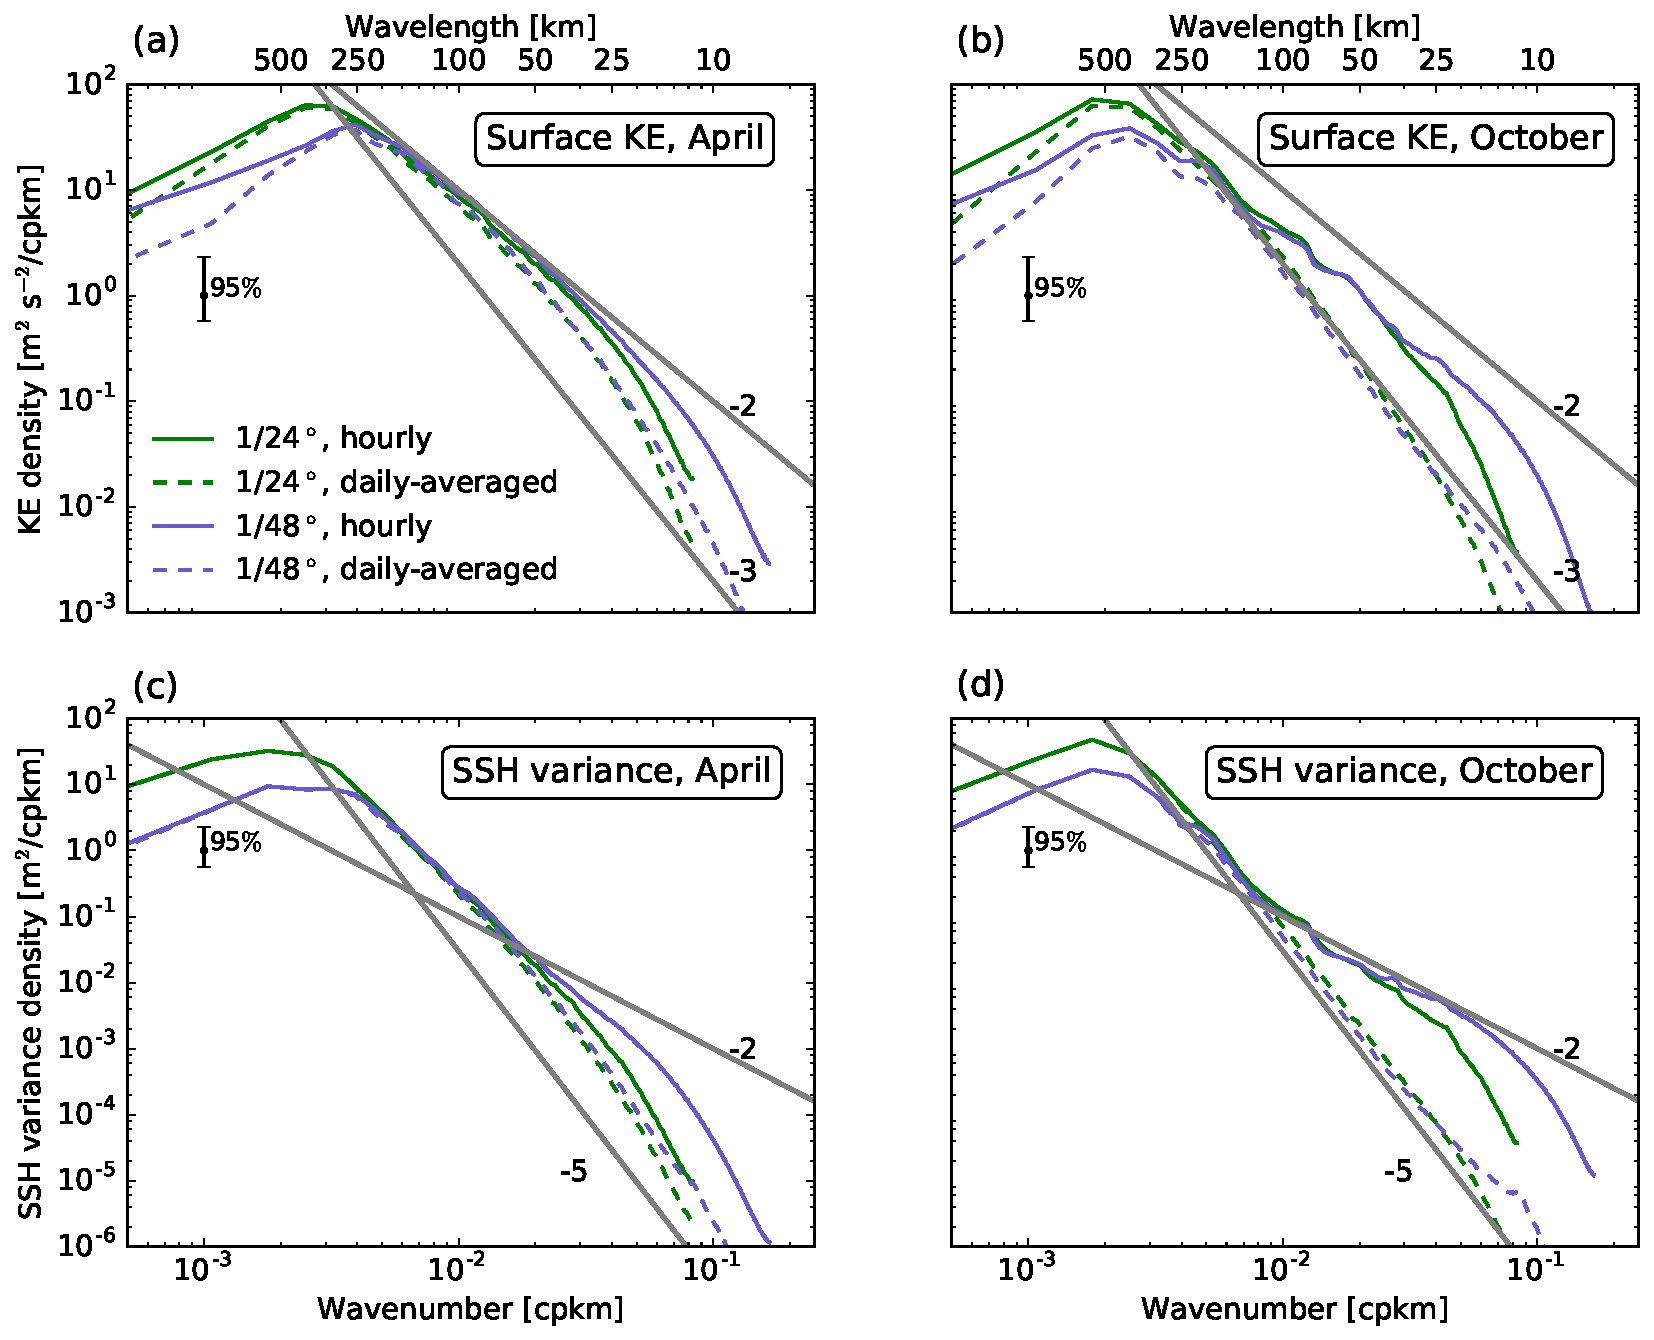
\includegraphics[width=40pc]{figs/fig_s2_3.pdf}
   \caption{A comparison between spectra of the two LLC simulations 1/24$^\circ$
   (green) and 1/48$^\circ$ (purple). The statistical errorbars represent conservative
   95$\%$ significance levels.  As expected the
   higher-resolution simulation (LLC4320) essentially extends the spectra of the
   lower-resolution simulation (LLC2160) towards smaller scale, demonstrating that
   the higher resolution is resolving a wider array of scales. Between 20 and 100 km
   the spectra of the two simulations are visually indistinguishable.}
   \label{figS2_3}
   \end{center}
 \end{figure}


 \begin{figure}
    \begin{center}
      \setfigurenum{S2}
      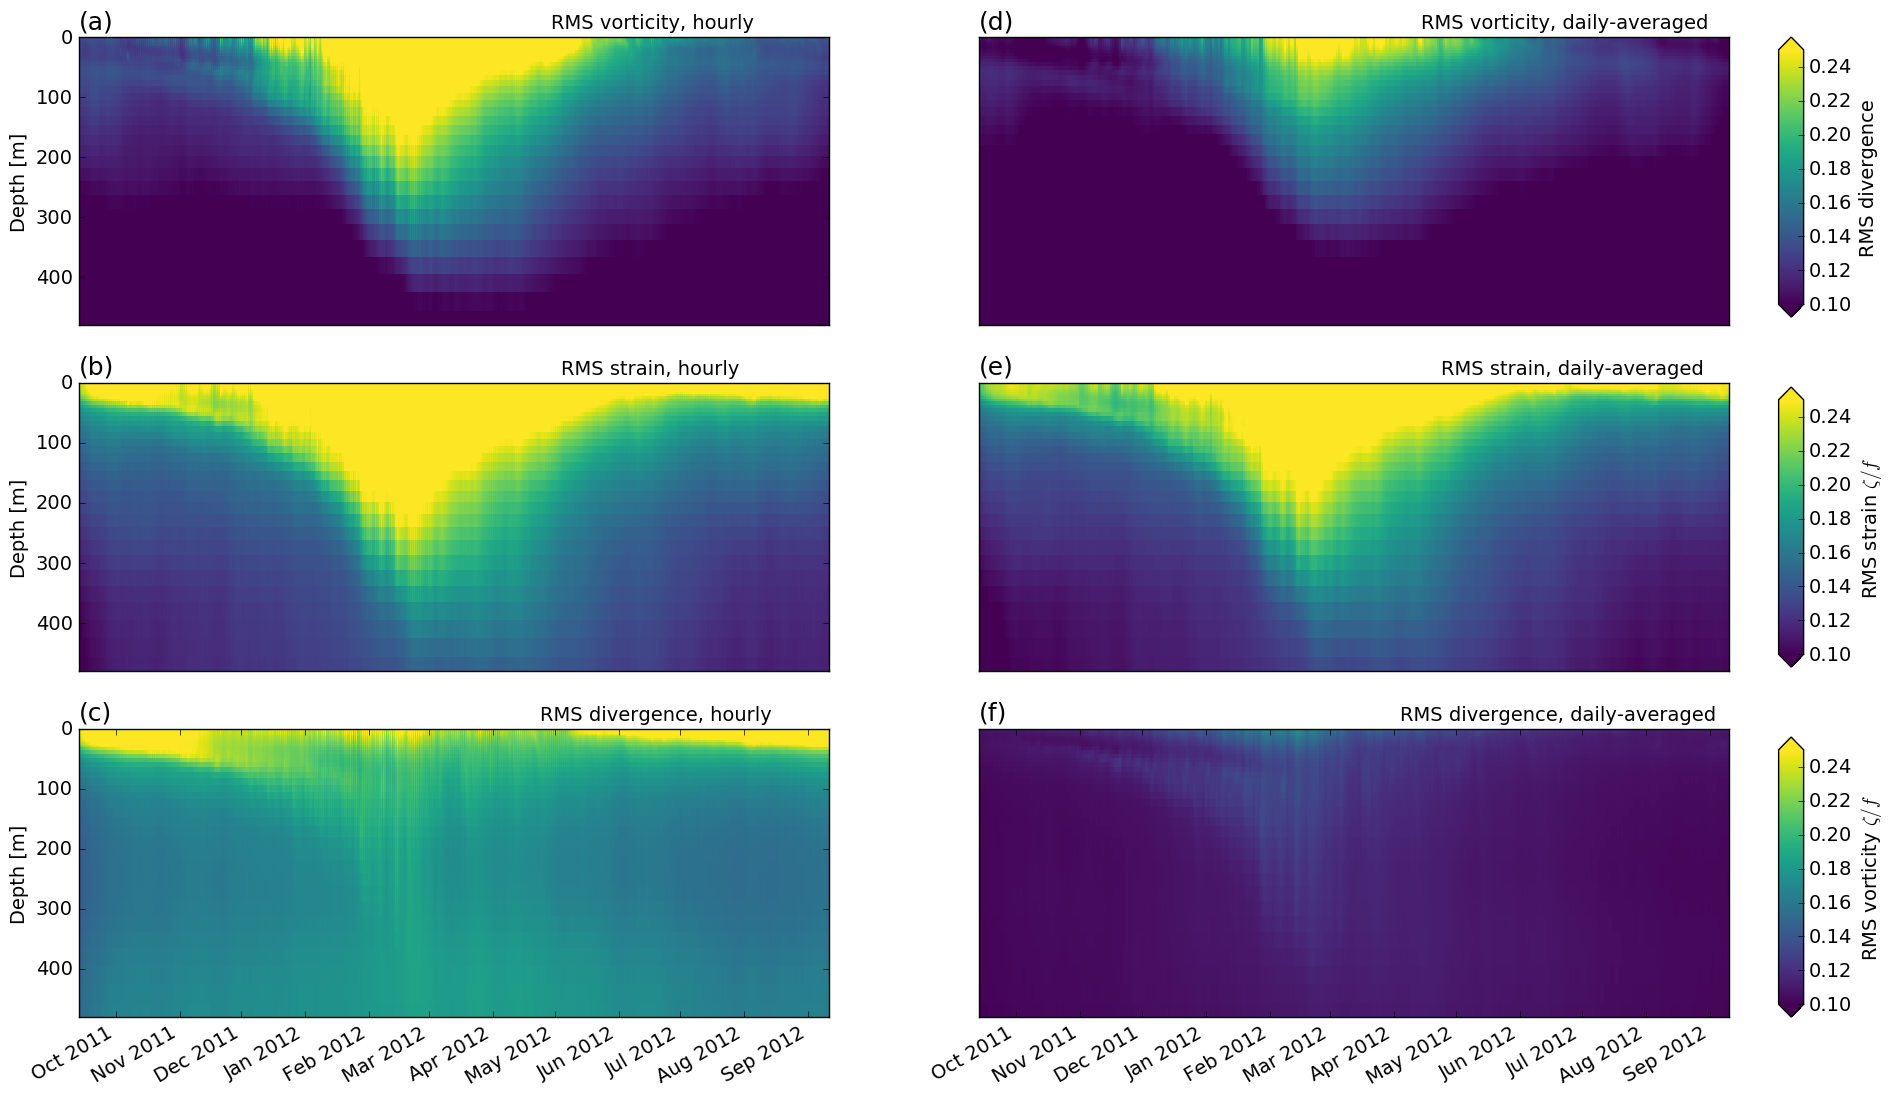
\includegraphics[width=40pc]{figs/fig_s2_2.pdf}
   \caption{Time dependence of probability density functions of vertical vorticity (a, b)
   and horizontal divergence (c, d). Monthly averages in April and October are
   also shown (e, f). The time series of vorticity PDF indicate that
   the development of positive skewness in winter (Figures \ref{figS2_2}a-b) both in
   hourly ($\sim 1.4$) and daily-averaged ($\sim1.1$) fields. The skewness
   in divergence for hourly fields is very small year-round ($\sim -0.24$), suggesting the
   prevalence of inertia-gravity waves. Filtering out the waves by daily-averaging
   the velocity field increases the skewness in divergence, particularly in winter ($\sim-0.64$). Both
  positive vorticity (cyclonic) skewness and negative divergence (convergence) skewness
  are characteristics of submesoscale turbulence.}
   \label{figS2_2}
   \end{center}
 \end{figure}

 \begin{figure}
    \begin{center}
      \setfigurenum{S3}
      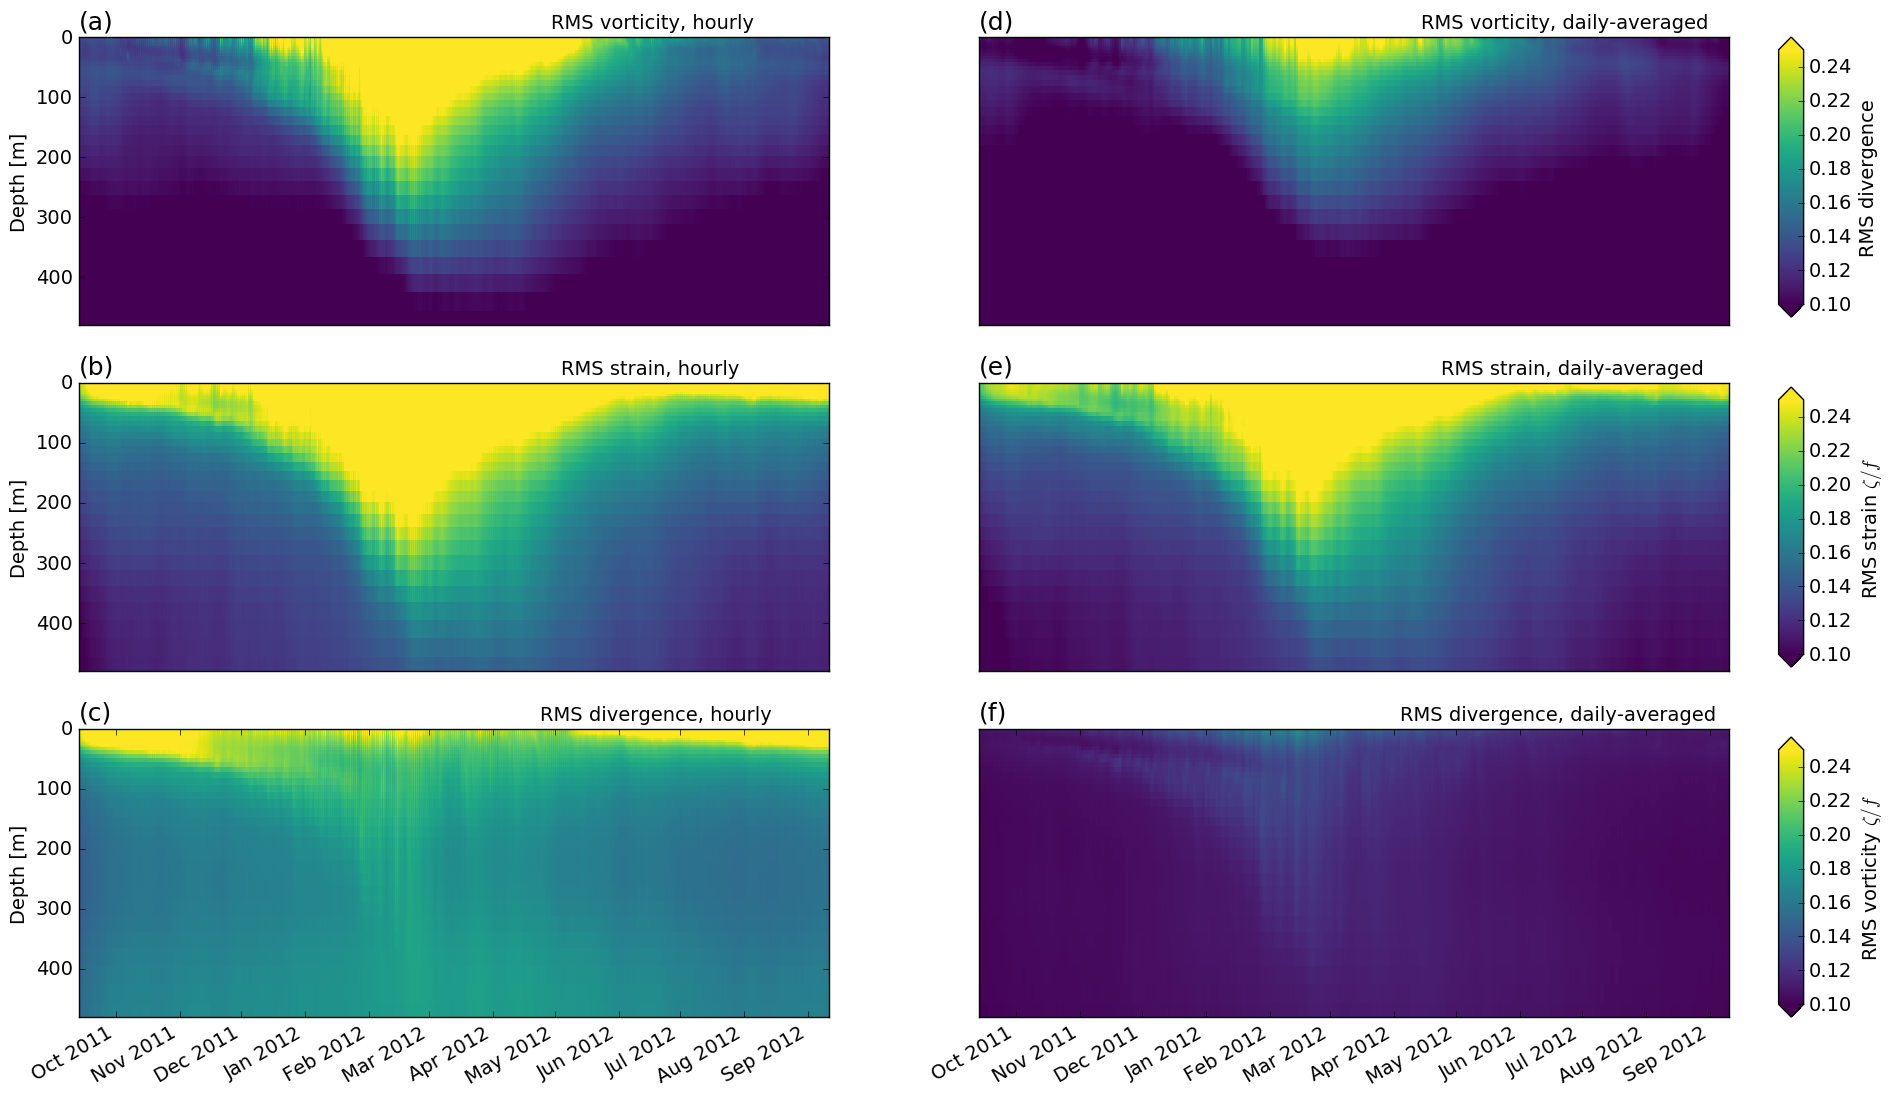
\includegraphics[width=40pc]{figs/fig_s2_2.png}
   \caption{Depth-dependence of root-mean-square of vertical vorticity (a,d), rate of lateral strain (b,e)
   and horizontal divergence (c,f) for hourly (a,b,c) and daily-averaged (d,e,f,) fields.
   The strong seasonality, as depicted
   at the surface in Figure 2 of the main manuscript, is confined to the mixed layer, which
   varies from 50 m in summer to about 350 m in winter.}
   \label{figS2_2}
   \end{center}
 \end{figure}

 \begin{figure}
    \begin{center}
      \setfigurenum{S4}
      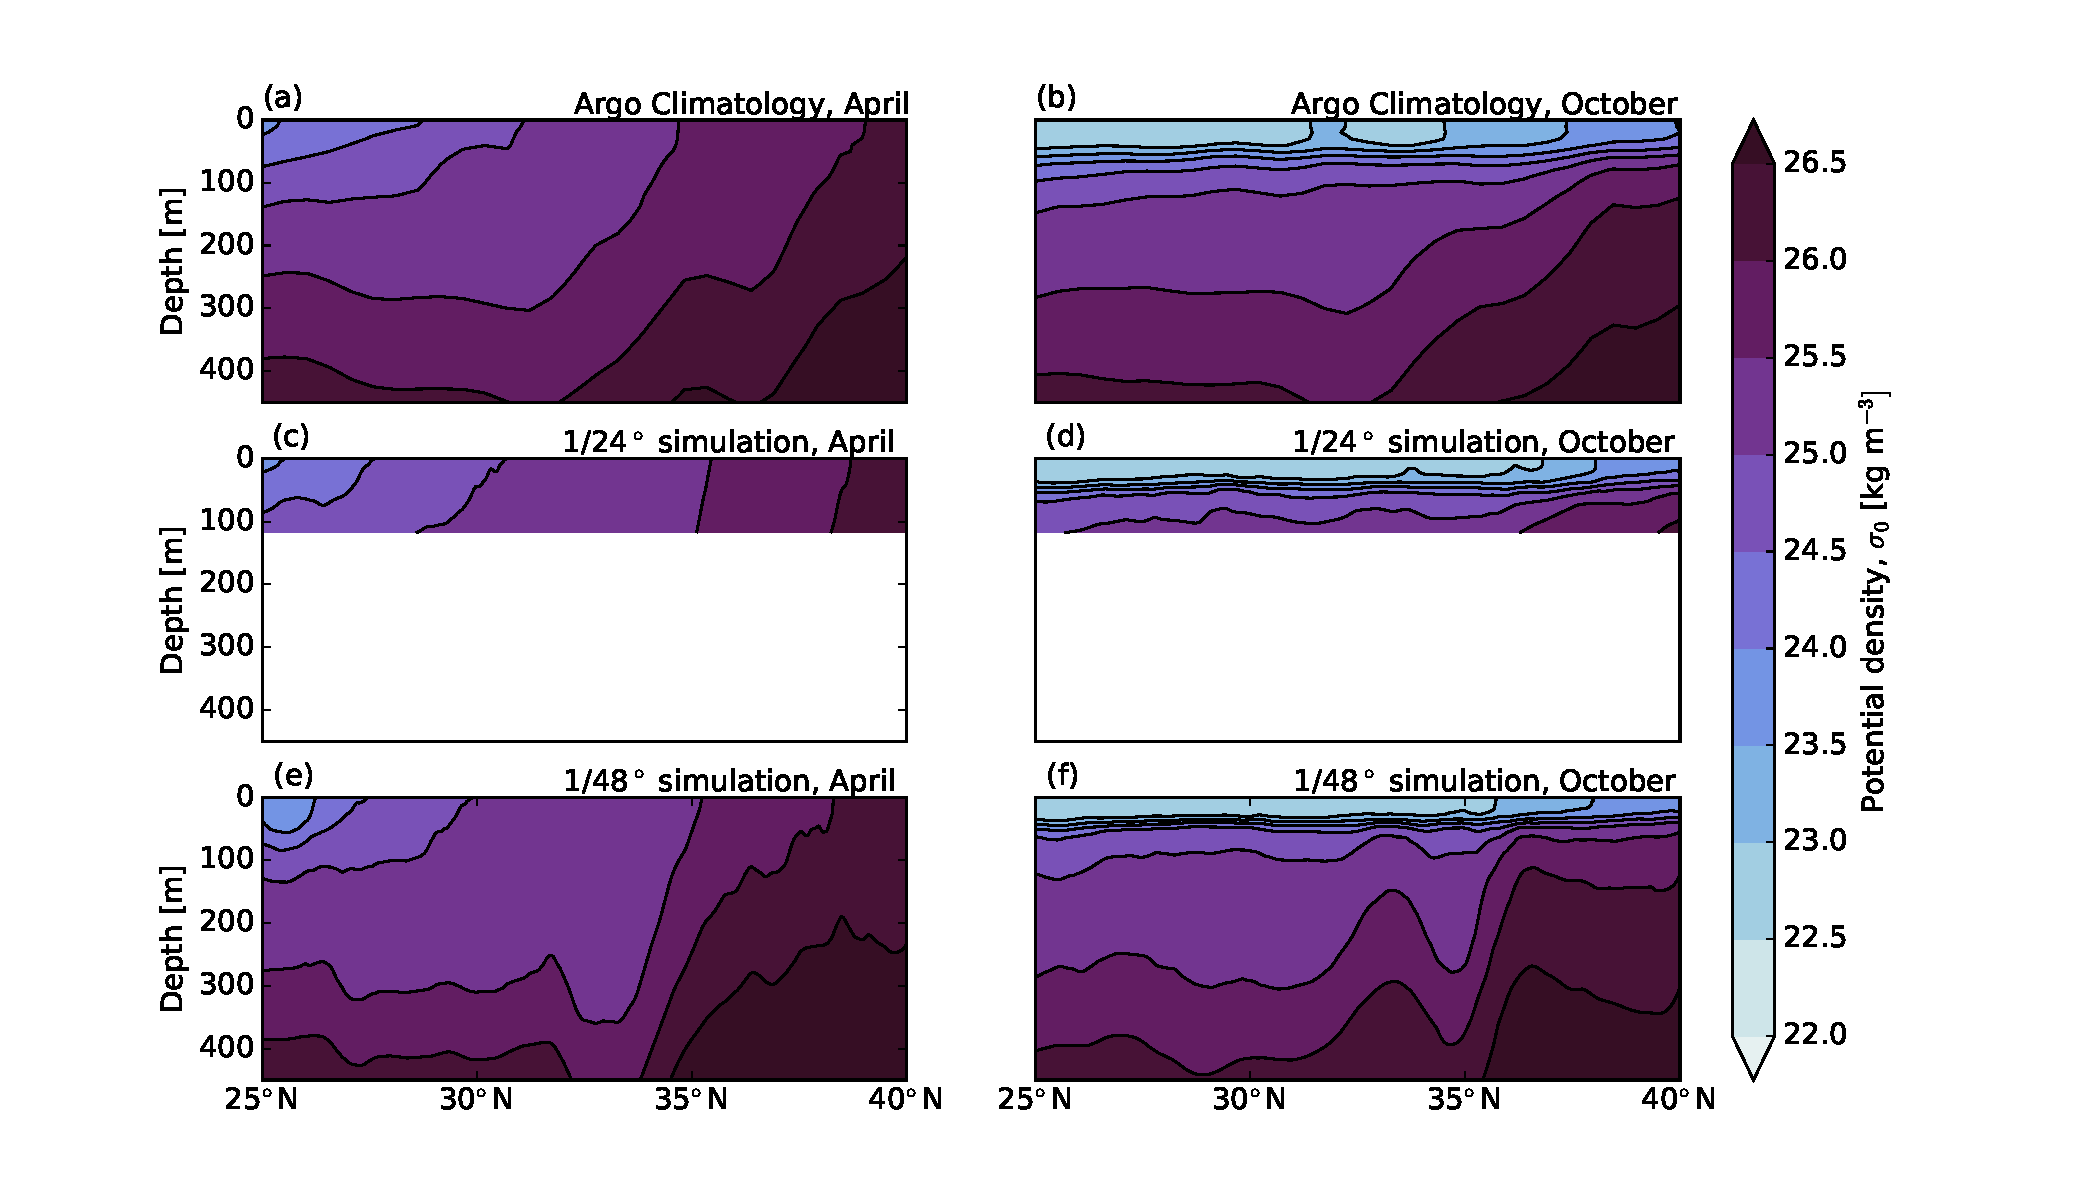
\includegraphics[width=40pc]{figs/fig_s2_1.pdf}
   \caption{Potential density: a comparison between Roemmich-Gilson Argo
           climatology [updates from \cite{roemmich_gilson2009}] (a, b) and the LLC simulations 1/24$^\circ$ (c, d)
           and  1/48$^\circ$ (e, f). Of course, the Argo climatology is smoother
           owing to lower resolution and long-term averaging. Nonetheless, simulations reproduce well the strong
           seasonality in the stratification. The upper ocean is weakly stratified in late winter/early fall
           and re-stratifies in summer. Argo climatology and LLC simulations mixed-layer depths are consistent
           at all seasons (not shown). The Argo climatology is available online at
           \texttt{http://sio-argo.ucsd.edu/RG\_Climatology.html}.}
   \label{figS2_1}
   \end{center}
 \end{figure}

 \begin{figure}
    \begin{center}
      \setfigurenum{S5}
      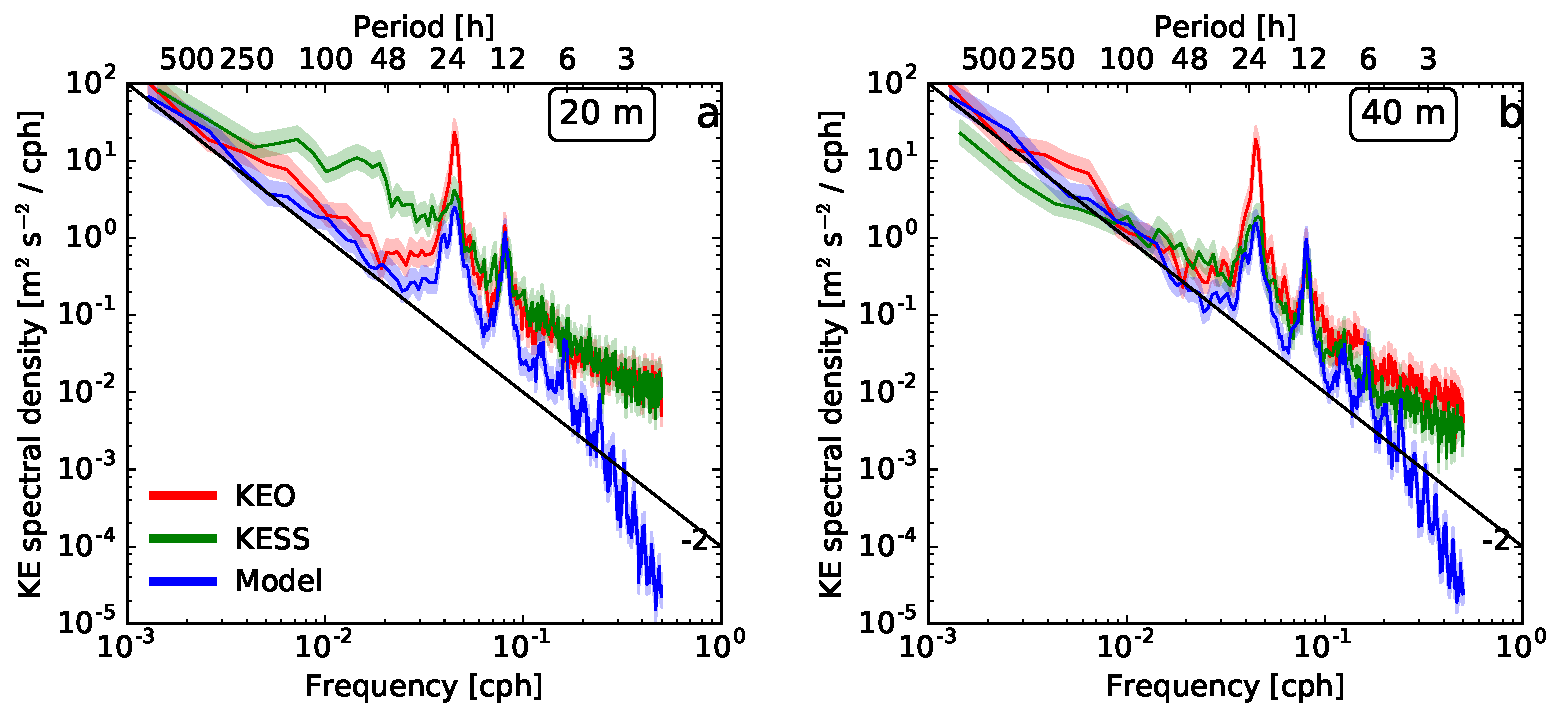
\includegraphics[width=40pc]{figs/figA1.pdf}
   \caption{A comparison between frequency spectra of LLC simulations and two
   available moored current meter records.}
   \label{figA1}
   \end{center}
 \end{figure}

 \begin{figure}
    \begin{center}
      \setfigurenum{S6}
      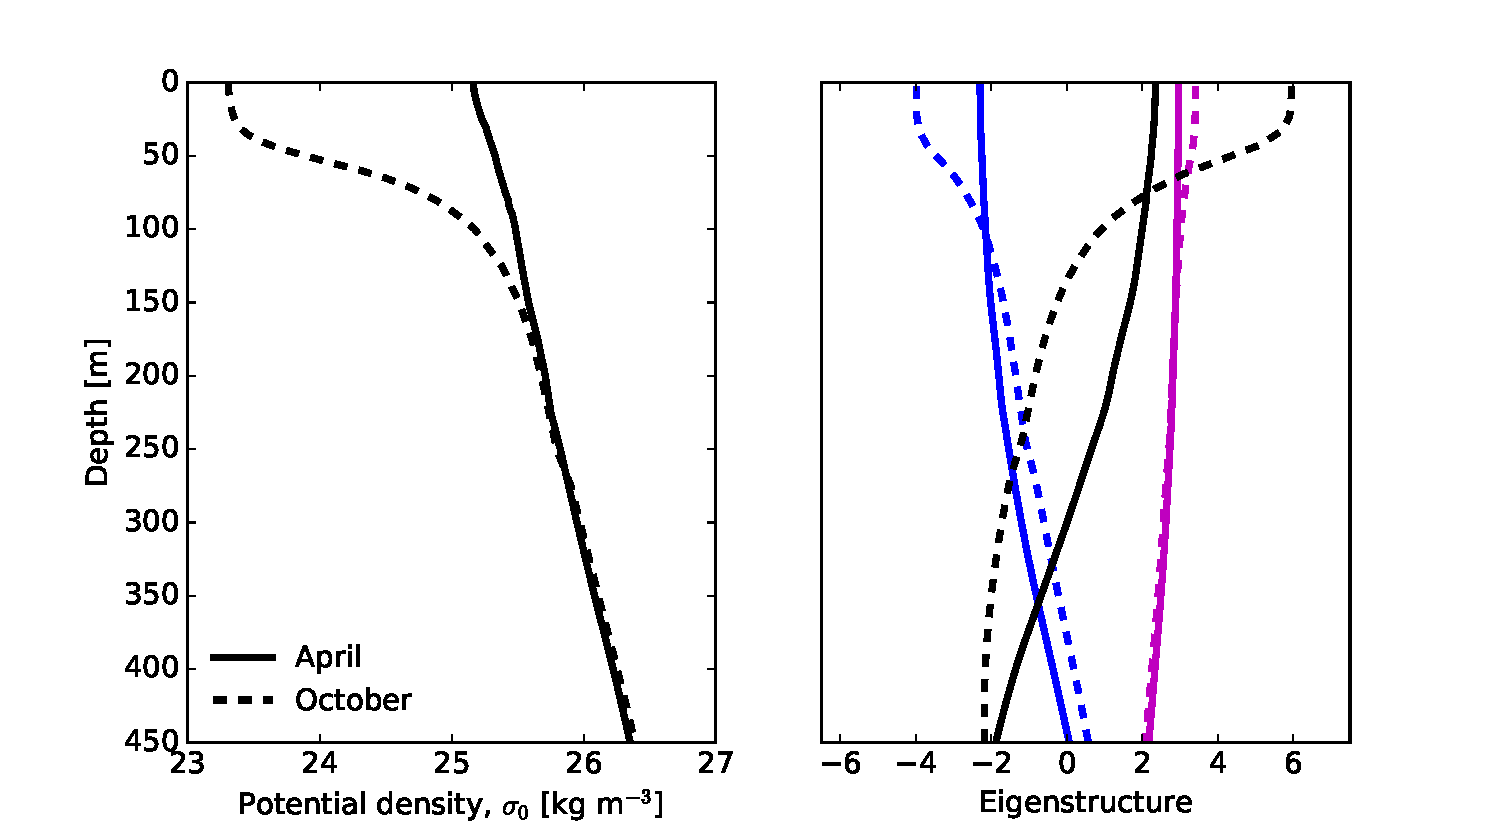
\includegraphics[width=40pc]{figs/fig_s3.pdf}
   \caption{The seasonal variability of the WOA 2013 \citep{levitus_etal2013} stratification averaged  over
   the domain and the associated three gravest pressure modes. Only the upper 450 m is shown.
   Clearly, the changes to the stratification
   are dramatic, with the formation of a seasonal pycnocline in summer. The strong
   seasonality of upper-ocean stratification yields a strong seasonality in the
   near-surface shape and amplitude of baroclinic pressure modes.
   In particular, the surface amplitude is much large in summer. Thus the projection
   of baroclinic tides on the surface may vary significantly seasonally. The WOA data is
   available online at \texttt{https://www.nodc.noaa.gov/OC5/woa13/}.}
   \label{figS3}
   \end{center}
 \end{figure}


 \begin{table}
 \label{tab:llc}
 \settablenum{S1}
 \caption{\small The MITgcm Latitute-Longitude Cap (LLC) spin-up hierarchy. This study analyzes
          the output of LLC2160 and LLC4320. Model fields are available hourly.
          Adapted from \cite{rocha_etal2016}.}
 \begin{center}
 \begin{tabular}{ | c | c | c | c | c |}
 \hline
 Simulation & Resolution & Time-step & Period  & Tides \\ \hline
 ECCO2 Adjoint & $1/6^{^\circ}$ & 1200 s & January 2009 - December 2011 & No\\
 LLC 1080   & $1/12^{^\circ}$ & 90 s & January 2010 - July 2012 & No\\
 LLC 2160   &  $1/24^{^\circ}$ & 45 s  & January 2011 - April 2013 & Yes\\
 LLC 4320   &  $1/48^{^\circ}$ & 25 s & September 2011 - September 2012 & Yes \\
 \hline
 \end{tabular}
 \end{center}
 \end{table}



% ---------------
% EXAMPLE TABLE
%
%\begin{table}
%\settablenum{S1} %%Change number for each table
%\caption{Time of the Transition Between Phase 1 and Phase 2\tablenotemark{a}}
%\centering
%\begin{tabular}{l c}
%\hline
% Run  & Time (min)  \\
%\hline
%  $l1$  & 260   \\
%  $l2$  & 300   \\
%  $l3$  & 340   \\
%  $h1$  & 270   \\
%  $h2$  & 250   \\
%  $h3$  & 380   \\
%  $r1$  & 370   \\
%  $r2$  & 390   \\
%\hline
%\end{tabular}
%\tablenotetext{a}{Footnote text here.}
%\end{table}
% ---------------
%
% EXAMPLE LARGE TABLE (UPLOADED SEPARATELY)
%\begin{table}
%\settablenum{S1} %%Change number for each table
%\caption{Time of the Transition Between Phase 1 and Phase 2\tablenotemark{a}}
%\end{table}


\end{document}

%%%%%%%%%%%%%%%%%%%%%%%%%%%%%%%%%%%%%%%%%%%%%%%%%%%%%%%%%%%%%%%

More Information and Advice:

%% ------------------------------------------------------------------------ %%
%
%  SECTION HEADS
%
%% ------------------------------------------------------------------------ %%

% Capitalize the first letter of each word (except for
% prepositions, conjunctions, and articles that are
% three or fewer letters).

% AGU follows standard outline style; therefore, there cannot be a section 1 without
% a section 2, or a section 2.3.1 without a section 2.3.2.
% Please make sure your section numbers are balanced.
% ---------------
% Level 1 head
%
% Use the \section{} command to identify level 1 heads;
% type the appropriate head wording between the curly
% brackets, as shown below.
%
%An example:
%\section{Level 1 Head: Introduction}
%
% ---------------
% Level 2 head
%
% Use the \subsection{} command to identify level 2 heads.
%An example:
%\subsection{Level 2 Head}
%
% ---------------
% Level 3 head
%
% Use the \subsubsection{} command to identify level 3 heads
%An example:
%\subsubsection{Level 3 Head}
%
%---------------
% Level 4 head
%
% Use the \subsubsubsection{} command to identify level 3 heads
% An example:
%\subsubsubsection{Level 4 Head} An example.
%
%% ------------------------------------------------------------------------ %%
%
%  IN-TEXT LISTS
%
%% ------------------------------------------------------------------------ %%
%
% Do not use bulleted lists; enumerated lists are okay.
% \begin{enumerate}
% \item
% \item
% \item
% \end{enumerate}
%
%% ------------------------------------------------------------------------ %%
%
%  EQUATIONS
%
%% ------------------------------------------------------------------------ %%

% Single-line equations are centered.
% Equation arrays will appear left-aligned.

Math coded inside display math mode \[ ...\]
 will not be numbered, e.g.,:
 \[ x^2=y^2 + z^2\]

 Math coded inside \begin{equation} and \end{equation} will
 be automatically numbered, e.g.,:
 \begin{equation}
 x^2=y^2 + z^2
 \end{equation}

% IF YOU HAVE MULTI-LINE EQUATIONS, PLEASE
% BREAK THE EQUATIONS INTO TWO OR MORE LINES
% OF SINGLE COLUMN WIDTH (20 pc, 8.3 cm)
% using double backslashes (\\).

% To create multiline equations, use the
% \begin{eqnarray} and \end{eqnarray} environment
% as demonstrated below.
\begin{eqnarray}
  x_{1} & = & (x - x_{0}) \cos \Theta \nonumber \\
        && + (y - y_{0}) \sin \Theta  \nonumber \\
  y_{1} & = & -(x - x_{0}) \sin \Theta \nonumber \\
        && + (y - y_{0}) \cos \Theta.
\end{eqnarray}

%If you don't want an equation number, use the star form:
%\begin{eqnarray*}...\end{eqnarray*}

% Break each line at a sign of operation
% (+, -, etc.) if possible, with the sign of operation
% on the new line.

% Indent second and subsequent lines to align with
% the first character following the equal sign on the
% first line.

% Use an \hspace{} command to insert horizontal space
% into your equation if necessary. Place an appropriate
% unit of measure between the curly braces, e.g.
% \hspace{1in}; you may have to experiment to achieve
% the correct amount of space.


%% ------------------------------------------------------------------------ %%
%
%  EQUATION NUMBERING: COUNTER
%
%% ------------------------------------------------------------------------ %%

% You may change equation numbering by resetting
% the equation counter or by explicitly numbering
% an equation.

% To explicitly number an equation, type \eqnum{}
% (with the desired number between the brackets)
% after the \begin{equation} or \begin{eqnarray}
% command.  The \eqnum{} command will affect only
% the equation it appears with; LaTeX will number
% any equations appearing later in the manuscript
% according to the equation counter.
%

% If you have a multiline equation that needs only
% one equation number, use a \nonumber command in
% front of the double backslashes (\\) as shown in
% the multiline equation above.

%% ------------------------------------------------------------------------ %%
%
%  SIDEWAYS FIGURE AND TABLE EXAMPLES
%
%% ------------------------------------------------------------------------ %%
%
% For tables and figures, add \usepackage{rotating} to the paper and add the rotating.sty file to the folder.
% AGU prefers the use of {sidewaystable} over {landscapetable} as it causes fewer problems.
%
% \begin{sidewaysfigure}
% \includegraphics[width=20pc]{samplefigure.eps}
% \caption{caption here}
% \label{label_here}
% \end{sidewaysfigure}
%
%
%
% \begin{sidewaystable}
% \caption{}
% \begin{tabular}
% Table layout here.
% \end{tabular}
% \end{sidewaystable}
%
%
